\documentclass[letterpaper,12pt]{article}
\usepackage{booktabs,graphicx,amssymb,lineno,amsmath,multirow,rotating,verbatim,setspace,float,subfigure, fixltx2e}
\usepackage[margin=1in]{geometry}
\usepackage{gensymb}
\usepackage[table]{xcolor}

%*******************************************************************************************************
% verbatim lets you do \begin{} and \end {} comment
%amsymb & amssymb useful for math.  
% check out the wiki page 
%/cite  or citep (with natbib package?)
%/textit or 

%added fixlt2e 

% Latex once to get the file
% Then bibtex (Put in the same WD)
% then typeset LaTex again by pushing typeset twice to get the citations in 

\begin{document}

\linenumbers
%\renewcommand{\thesubfigure}{\Alph{subfigure}}
%\bibpunct{[}{]}{,}{n}{,}{,}

\title{Summary of BTB-brucellosis coinfection model and assumptions}
\date{23-April-2016}

\maketitle
%\singlespace
\doublespacing

\section*{Overview}
Bovine tuberculosis (bTB) and brucellosis are positively associated at the population level.   Age prevalence curves show a shift in the peak age of brucellosis infection in co-infected animals (Figure 1).  We want to know why, so we investigate the costs of co-infection on three parameters relevant for disease dynamics. \\
1. \textit{Host mortality rates}: bTB was associated with a 2.81 ($95\% CI 1.47-6.82$) fold increase in mortality hazard and infection with brucellosis was associated with an 3.00 ($95\% CI 1.50-6.01$) fold increase in mortality hazard compared to uninfected buffalo.  We did not find support for an interaction between bTB and brucellosis on mortality, indicating that the mortality effects of both infections are additive in co-infected buffalo.   \\
2. \textit{Incidence rates}:  bTB was associated with a 1.37 fold increase in the rate at which animals acquire brucellosis.  This pattern occurred in one site but not the second.  I think this is because the higher baseline mortality in the second site means we do not catch and diagnose infected individuals before they die and hope to test this with the model.\\
3. \textit{Pregnancy rates}:  We see declines in pregnancy rates with infection.  However, buffalo population dynamics are more rainfall driven than disease driven (Cross et al. 2009), so we consider density dependence in births following Gao and Hethcote 1992.\\

The model then asks, (1) are changes in these rates sufficient to generate the positive co-infection patterns observed and (2) what is the consequence of brucellosis infection for the invasion of bTB? and (3) what is the consequence of bTB invasion for the dynamics of brucellosis (endemic equilibrium values). 

\begin{figure}
\begin{center}
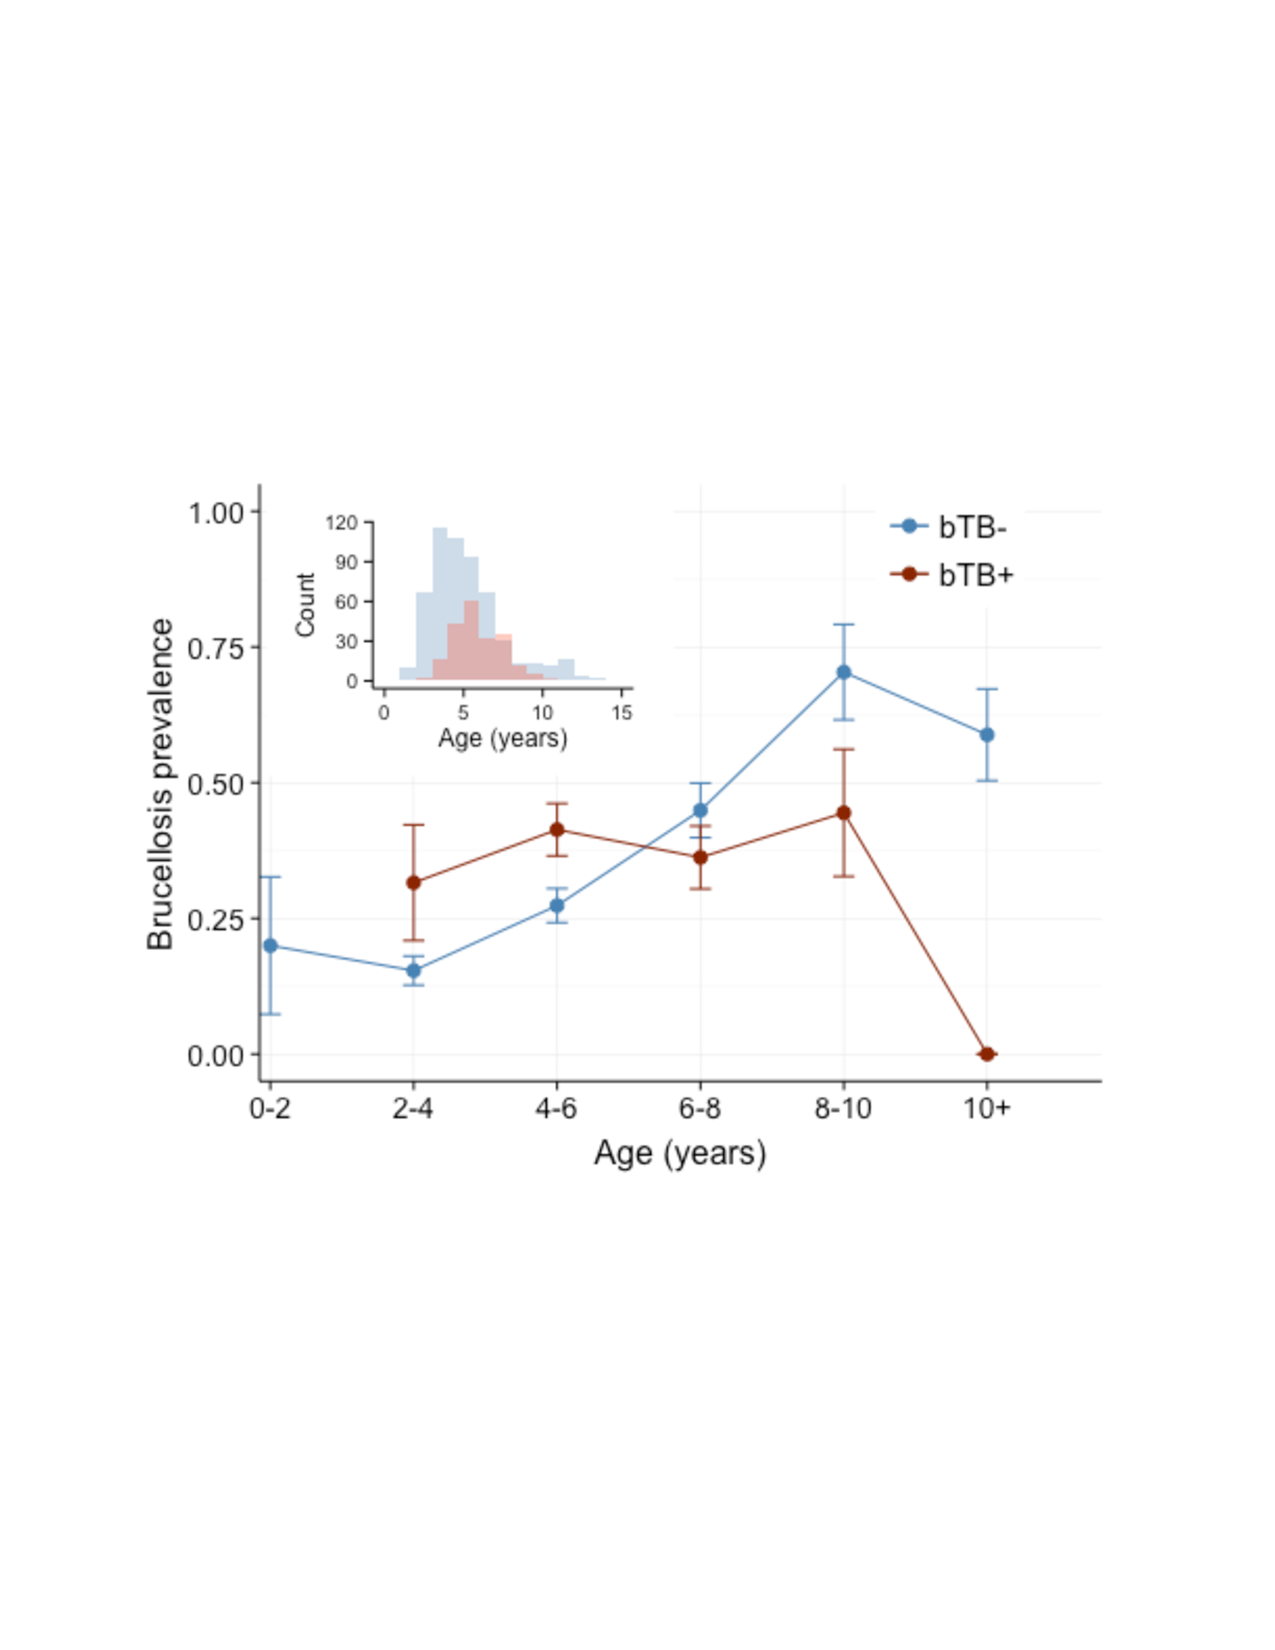
\includegraphics[width=5in]{Figure1_ageprev}
\end{center}
\caption{Age, brucellosis-prevalence curves in buffalo simultaneously uninfected (blue) or infected (red) with bTB.  The inset figure shows the distribution of ages in our sample, which best cover buffalo between two and eight years old and include 796 samples from 151 repeatedly captured individuals.  Ages are binned for visualization and animals that test positive are assumed to remain positive for the duration of the study.  Sample sizes for TB- are: 10, 182, 209, 103, 27, 35 buffalo.  Sample sizes for TB+ animals are: 0, 21, 108, 75, 21, 1 for ages 0-2, 2-4, 4-6, 6-8, 8-10, and 10+ respectively.}
\label{fig1}
\end{figure}

%%%%%%%%NOTE%%%%%%%%%%
% Think about last data point. % Maybe remove 10+ TB positive point, put large CI on it. 

\pagebreak
\section*{Model Structure and Assumptions}
\indent
	We developed a continuous time differential equation model to evaluate the disease dynamic consequence of bTB invasion on brucellosis dynamics and vice versa.  
Our model structure reflects the costs of co-infection identified for each parameter: host mortality rate, host birth rate, and disease transmission rates (Figure 2).
Animals are represented with six groups: susceptible to both infections($S$), acutely infected with brucellosis ($I_{B}$), chronically infected with or recovered from acute brucellosis ($R_{B}$), infected with bTB ($I_{T}$), co-infected with both pathogens ($I_{C}$), or in the chronic stages of brucellosis and infected with bTB ($R_{C}$).  These assumptions give the following set of 6 differential equations: 
\begin{figure}
\begin{center}
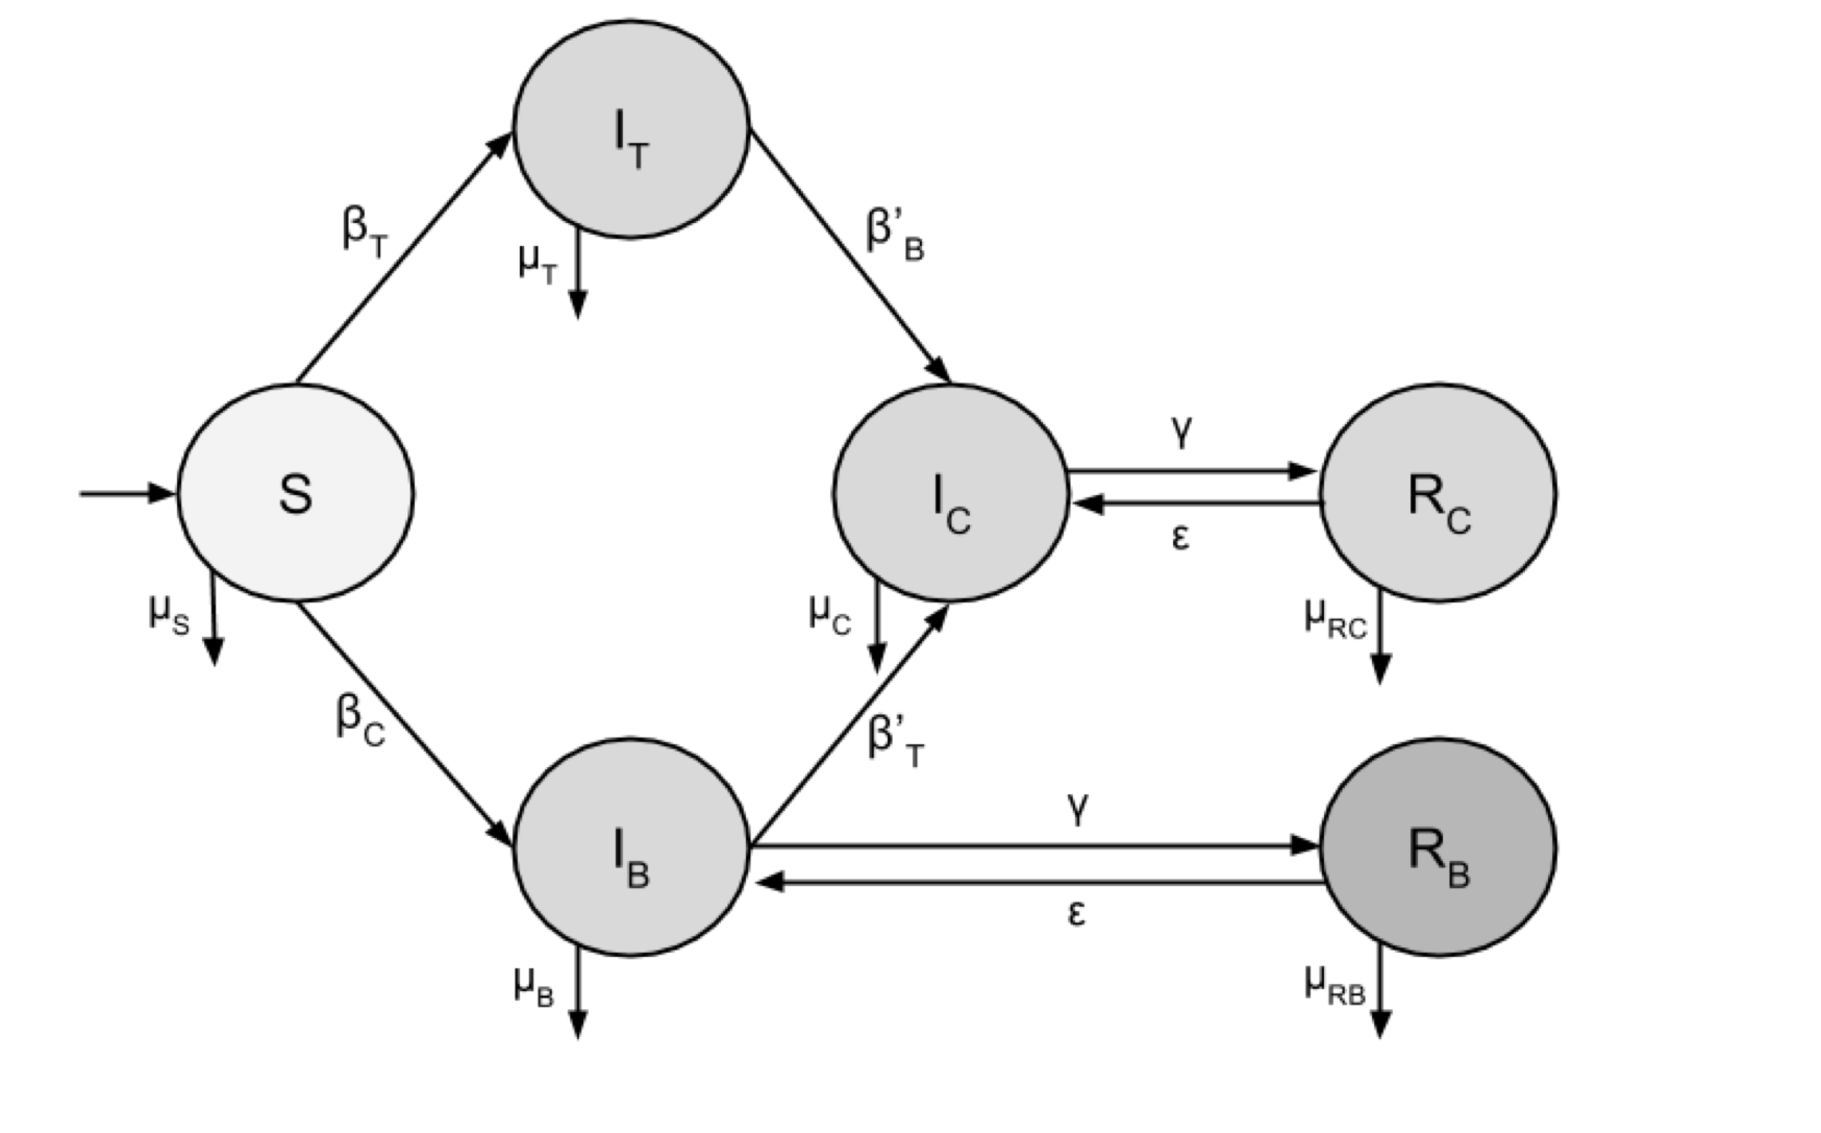
\includegraphics[width=5in]{bTB_Bruc_model}
\end{center}
\caption{Diagram of model structure and assumptions.  
We model bTB infection as a directly transmitted, lifelong infection (Bengis 1999).  
We model brucellosis infection as a persistent infection, by allowing animals to recrudesce and transmit the infection.
Buffalo populations experience logistic growth with density dependence in births rates that are independent of disease and for a fixed carrying capacity, K (Gao and Hethcote 1992).
Transmission of both infections are assumed to be density dependent.}
\label{fig2}
\end{figure}
% Maybe need to highlight the framework more- We incorporate uncertainty associated with the effects of infection and co-infection on host survival and disease transmission by simulating infection dynamics directly from posterior estimates from our statistical models.   
%%%%%%%%%%%%%%%%%%%%%%%%%%%%%%%%%%%%
%%%%%%%%%%%%%%%%%%%%%%%%%%%%%%%%%%%%
%Attempt 3 with density dependent births and death rates, no age categories
%%%%%%%%%%%%%%%%%%%%%%%%%%%%%%%%%%%%
%%%%%%%%%%%%%%%%%%%%%%%%%%%%%%%%%%%%
\begin{align*}
N & = S + I_{T} + I_{B} + R_{B} + I_{C} + R_{C} \\
T &= I_{T} + I_{C} + R_{C} \\
B &= I_B+I_C \\
N_{b} &= S + b_1 I_{T}+ b_2 I_{B} + b_3 R_{B} + b_4 I_{C} + b_5 R_{C} \\
\frac{dS}{dt} &= b N_b \big(1 - \frac{r}{b} \frac{N}{K}\big) - \beta_T T S - \beta_B B S - \mu_{S} S  \\		      			% Susceptibles 
\frac{dI_{T}}{dt}&= \beta_T T S -  \beta'_{B} B I_{T} - \mu_{T} I_{T} \\									% TB 
\frac{dI_{B}}{dt}&=  \beta_B B S - \beta'_T T I_{B} - \gamma I_{B} + \epsilon R_{B}  - \mu_{B} I_{B} \\ 		 	% Brucellosis
\frac{dI_{C}}{dt}&=  \beta'_T T I_{B} + \beta'_{B} B I_{T} - \gamma I_{C} + \epsilon R_{C}  - \mu_{C} I_{C}  \\  		% Co-infecteds 
\frac{dR_{B}}{dt}&=  \gamma I_{B} - \epsilon R_{B} - \mu_{RB} R_{B} \\  												% Chronic brucellosis 
\frac{dR_{C}}{dt}&=  \beta'_T T R_{B} + \gamma I_{C} - \epsilon R_{C} - \mu_{R_{C}} R_{C} \\ 						% Chronic Brucellosis and co-infecteds
\end{align*}

where $N$ is the total host population and T, B, and $N_b$ are the numbers of buffalo contributing to tuberculosis transmission, brucellosis transmission, and births respectively. \\

To evaluate the consequences of co-infection for disease invasion, we evaluate how co-infection alters the basic reproduction number ($R_{o}^{T}$) of bTB. \\
Lets first consider the bTB only model: 
\begin{align*}
\frac{dS}{dt}&=b (S + b_1 I_T)\left(1-\frac{r}{b}\frac{S+I_T}{K}\right) -\beta_T S I_T - \mu S\\
\frac{dI_T}{dt}&=\beta_T S I_T - \mu_{T} I_T
\end{align*}

$R_{o}^{T}$ for bTB in the case when brucellosis is absent is, $R_{o}^{T} = \frac{\beta_T K}{\mu_T}$.  
The disease free equilibrium is $E_o = (K, 0)$, where the variables are denoted $x_o = (S, I_T)$.
The endemic equilibrium for bTB when brucellosis is absent is,  $E^{*} = (S_{T}^{*}, I_{T}^{*})$, where $S_{T}^{*} = K \frac{1}{R_{o}^{T}}$ and 
\begin{equation*}
I_{T}^*=\frac{K}{2}\frac{1}{b_1}\left[ 
\left(\frac{bb_1 - \mu - \alpha_T}{r}  - \frac{1+b_1}{\mathcal{R}_0^{T}}\right) + \sqrt{\left(\frac{bb_1 - \mu - \alpha_T}{r}  - \frac{1+b_1}{\mathcal{R}_0^{T}}\right)^2 + 4 \frac{b_1 }{\mathcal{R}_0^{T}}\left(1-\frac{1}{\mathcal{R}_0^{T}}\right)}\right].
\end{equation*}

Now consider the brucellosis only model: 
\begin{align*}
\frac{dS}{dt} &= b (S+ b_2 I_{B} + b_3 R_{B}) \big(1 - \frac{r}{b} \frac{(S+ I_{B} + R_{B})}{K}\big)- \beta_B I_B S - \mu_{S} S  \\		      					% Susceptibles 
\frac{dI_{B}}{dt}&=  \beta_B I_B S - \gamma I_{B} + \epsilon R_{B}  - \mu_{B} I_{B} \\ 		 					% Brucellosis
\frac{dR_{B}}{dt}&=  \gamma I_{B} - \epsilon R_{B} - \mu_{RB} R_{B} \\  										% Chronic brucellosis 
\end{align*}

$R_{o} ^B$ for brucellosis in the case that bTB is absent is, $R_{o}^{B} = \frac{\beta_B K (\epsilon + \mu_R)}{(\gamma + \mu_B) (\epsilon + \mu_{RB}) + \epsilon \gamma}$ \\
The endemic equilibrium for brucellosis when bTB is absent is $E* = (S_{t}^*, I_{Bt}^*, R_{Bt}^*)$, where 
$S_{t}^* = \frac{K}{R_{o} ^B}$, \\
$I_{Bt}^* = \frac{K}{2} \frac{1}{b_2(1+\delta)+ b_3 (\delta + \delta^2)} + \Big[b b_2 + b b_3 \delta - \frac{ \beta_B K}{R_o} - \frac{r + r \delta + b_2 + b_3 \delta}{R_o}\Big] +\\
 \sqrt{4 + \frac{K}{b_2 (1-\delta) + b_3 (\delta + \delta^2)} \Big[b b_2 + b b_3 \delta - \frac{ \beta_B K}{R_o} - \frac{r + r \delta + b_2 + b_3 \delta}{R_o}\Big] ^2}$,\\
$R_{Bt}^* =  \frac{\gamma I_{Bt}^*}{\epsilon - \mu_R}$. \\
$R_o$ for bTB when brucellosis is present is evaluated at these conditions, where $\delta = \frac{\gamma}{\epsilon - \mu_R}.$
$R_{o}^{T} = 2$. \\
CHECK THIS WITH NUMERICAL INTEGRATION!!


\pagebreak 
\noindent
\textbf{Notes on deriving $R_{o}^{T}$}: \\
 $1.$ Note there are $n = 6$ components of this model, $m = 3$ of which are infected with bTB.  Define the vector, $x_o = [I_T, I_C, R_C, S, I_B, R_B]^T$, such that $x_i$ contains the huber of individuals in each component. \\
 $2. $  The rate of change of $x_i$ (e.g. the differential equations) can be represented as, $\mathcal{F}_i(x) - \mathcal{V}_i (x)$.  
 Here $\mathcal{F}_i (x)$ is the rate of appearance of new infections in compartment i and $\mathcal{V}_i (x)$ is the rate of transfer by all other means. 
Noting the negative sign with $\mathcal{V}_i (x)$ and that $\mathcal{F}_i (x)$ only includes infections that are newly arising and does not include terms which describe the transfer of infectious individuals from one infected compartment to another. \\
 Here, $\mathcal{F}_i (x) = \Big[\frac{\beta_T S (I_t + I_C+ R_C)}{S + I_T + I_B + I_C + R_B + R_C}$, $\frac{\beta_{T} I_B (I_t + I_C+ R_C)}{S + I_T + I_B + I_C + R_B + R_C}$, $\frac{\beta_{T} R_B (I_t + I_C+ R_C)}{S + I_T + I_B + I_C + R_B + R_C}, 0, 0, 0\Big]^T$. \\
  $\mathcal{V}_i (x) =\Big[ 2 \Big]^T$ \\
$3.$ Check $\mathcal{F}_i$ and $\mathcal{V}_i$ meet the conditions outlined by van den Driessche and Watmough (2002) so you can use the next generation matrix,  $FV^{-1}$, from m by m matrices of partial derivatives of $F_i$ and $V_i$.   (CHECK ME)
$F_i = \Big[\frac{\partial \mathcal{F}_i (x_o)}{\partial x_i} \Big]$.  $V_i = \Big[\frac{\partial \mathcal{V}_i (x_o)}{\partial x_i} \Big]$.  $x_o$ are the disease free equilibrium values of x.\\
$4.$ Define bTB free equilibrium values $x_o = [I_T = 0, I_C = 0, R_C = 0, S = S*, I_B= I_B*, R_B = R_B*]^T$.  Where $S*$, $I_B*$, and $R_B*$ are the equilibrium values of brucellosis in the absence of bTB.  \\
$5.$ Evaluate the F and V matrices at $x_o$.  \\
Here, $F_i = \begin{bmatrix} \frac{\beta_T S*}{(S* + I_B* + R_B*)} & \frac{\beta_T S*}{(S* + I_B* + R_B*)} & \frac{\beta_T S*}{(S* + I_B* + R_B*)} \\ 
\frac{\beta'_T I_B*}{(S* + I_B* + R_B*)}  & \frac{\beta'_T I_B*}{(S* + I_B* + R_B*)} & \frac{\beta'_T I_B*}{(S* + I_B* + R_B*)} \\
\frac{ \beta'_T R_B*}{(S* + I_B* + R_B*)} & \frac{ \beta'_T R_B*}{(S* + I_B* + R_B*)} & \frac{ \beta'_T R_B*}{(S* + I_B* + R_B*)} \end{bmatrix}$ \\
Here, $V_i = \begin{bmatrix} a&b&c \\ d&e&f \\ g&h&i \end{bmatrix}$ \\
$6.$ Calculate $FV^{-1}$ \\
$7.$ The dominant eigenvalue of $FV^{-1}$ is xxx. \\



%%%%%%%%%%%%%%%%%%%%%%%%%%%%%%%%%%%%
%%%%%%%%%%%%%%%%%%%%%%%%%%%%%%%%%%%%
%Attempt 2 with density dependent births and death rates, 2 age categories...
%%%%%%%%%%%%%%%%%%%%%%%%%%%%%%%%%%%%
%%%%%%%%%%%%%%%%%%%%%%%%%%%%%%%%%%%%

%\begin{align*}%[hb]
%N & = S_j + S_a + I_{T_j} + I_{T_a} + I_{B_j} + I_{B_a} + I_{C_j} + I_{C_a} + R_{B_j} + R_{B_a} + R_{C_j} + R_{C_a} \\
%N_{birth_u} &= S_a+b_1 I_{T_a}+ b_3 R_a + b_5 R_{C_a} \\
%N_{birth_b} &= b_2 I_{B_a} + b_4 I_{C_a}\\
%\lambda_T &= \frac{ \beta_T \big(I_{T_j} + I_{T_a} + I_{C_j} + I_{C_a} + R_{C_j} + R_{C_a}\big)}{N} \\
%\lambda'_{T} &= \frac{ \beta'_T \sum_{i=1}{4} (I_{T_i} + I_{C_i} + R_{C_i})}{N} \\
%\lambda_B &= \frac{\beta_B \sum_{i=1}^{4} (I_B+I_C)}{N} \\
%\lambda'_{B} &= \frac{\beta'_{B} \sum_{i=1}{4} (I_B+I_C)}{N} \\
%\end{align*}

%juvenile buffalo: 
%\begin{align*}
%\frac{dS_j}{dt} &= (b - r \frac{N}{K}) N_{birth_u} - \lambda_T S_j - \lambda_B S_j - \mu_{S_j} S_j - \nu S_j\\       	% Susceptible Juvenile
%\frac{dI_{T_j}}{dt}&= \lambda_T S_j -  \lambda'_{B} I_{T_j} - \mu_{T_j} I_{T_j} - \nu I_{T_j} \\					% TB juvenile
%\frac{dI_{B_j}}{dt}&= (b - r \frac{N}{K}) N_{birth_b} +  \lambda_B S_j - \lambda'_T  I_{B_j} - \gamma I_{B_j} + \epsilon R_{B_j} - \mu_{B_j} I_{B_j} - \nu I_{B_j}  \\	 % Brucellosis juveniles
%\frac{dI_{C_j}}{dt}&=   \lambda'_T I_{B_j} + \lambda'_B I_{T_j} - \gamma I_{C_j} + \epsilon R_{C_j}  - \mu_{C_j} I_{C_j} - \nu I_{C_j} \\  		  % co-infected juveniles
%\frac{dR_{B_j}}{dt}&= \gamma I_{B_j} - \epsilon R_{B_j} - \mu_{R_{B_j}} R_{B_j} - \nu R_{B_j} \\  			% Chronic brucellosis juveinles
%\frac{dR_{C_j}}{dt}&= \lambda'_T R_{B_j} + \gamma I_{C_j} - \epsilon R_{C_j} - \mu_{R_{C_j}} R_{C_i} -  \nu R_{C_j}\\ 		% Chronic brucellosis and co-infected juveinles
%\end{align*}

%adult buffalo: 
%\begin{align*}
%\frac{dS_a}{dt} &= \nu S_j - \lambda_T S_a - \lambda_B S_a - \mu_{S_a} S_a  \\		      			 	% Susceptible Adult
%\frac{dI_{T_a}}{dt}&= \nu I_{T_j} + \lambda_T S_a -  \lambda'_{B} I_{T_a} - \mu_{T_a} I_{T_a} \\	% TB adults
%\frac{dI_{B_a}}{dt}&=  \nu I_{B_j} + \lambda_B S_a - \lambda'_T  I_{B_a} - \gamma I_{B_a} + \epsilon R_{B_a}  - \mu_{B_a} I_{B_a}   \\ 		 % Brucellosis adults
%\frac{dI_{C_a}}{dt}&=  \nu I_{C_j} + \lambda'_T I_{B_a} + \lambda'_B I_{T_a} - \gamma I_{C_a} + \epsilon R_{C_a}  - \mu_{C_a} I_{C_a}  \\  		  % co-infected adults
%\frac{dR_{B_a}}{dt}&= \nu R_{B_j} + \gamma I_{B_a} - \epsilon R_{B_a} - \mu_{R_{B_a}} R_{B_a} \\  		% Chronic brucellosis adults
%\frac{dR_{C_a}}{dt}&= \nu R_{C_j} + \lambda'_T R_{B_a} + \gamma I_{C_a} - \epsilon R_{C_a} - \mu_{R_{C_a}} R_{C_a} \\ 	% Chronic brucellosis and co-infected adults
%\end{align*}

%where $N$ is the total host population, $N_{birth_u}$ and $N_{birth_b}$ are the number of buffalo contributing uninfected and brucellosis infected births, and $\lambda_T, \lambda_B, \lambda'_{T}, \lambda'_{B}$ represent the force of infection for TB or brucellosis in susceptible buffalo ($\lambda_T, \lambda_B$) and buffalo with a previous infection ($\lambda'_{T}, \lambda'_{B}$)\\

% JAN MEETING NOTES... TRY TO PUT BIRTHS AND INPUTS ABOVE TO REDUCE THE NUMBER OF EQUATIONS
% OR PUT IN SAME ORDER WITH NU ALWAYS AT THE END!


%\pagebreak
%\begin{table}[hb]
%\small
%\newcommand{\head}[1]{\textnormal{\textbf{#1}}}
%\begin{tabular}{l l}
%\hline
%\textbf{Variable} & \textbf{Definition} \\
%\hline
%$S_i$ & Number of susceptible buffalo in age category, $i =$ juvenile, adults. \\
%$I_{T_i}$ & Number of buffalo infected with bTB  \\
%$I_{B_i}$ & Number of buffalo infected and infectious with brucellosis \\ 
%$I_{C_i}$ & Number of co-infected buffalo \\
%$R_{B_i}$ & Number of buffalo in the chronic stages of brucellosis \\
%$R_{C_i}$ & Number of buffalo in the chronic stages of brucellosis with bTB \\
%N & Total number of individuals \\
%\hline 
%\end{tabular}
%\label{table 1:}
%\caption{Notation used to denote model variables.  
%Variables with subscripts reflect juvenile (aged $\leq4$ yr) vs. adult age categories ($5+$)}
%\end{table}





\pagebreak
%\begin{align*}%[hb]
%N=& \sum_{i=1} ^{4} S_i+I_{T_i}+I_{B_i}+ I_{C_i}+ C_{B_i} + C_{C_i} \\
%N_{b}=& \sum_{i=1} ^{4} S_i+b_{1_i} I_{T_i}+ b_{2_i} I_{B_i}+ b_{3_i} I_{C_i} + C_{B_i} + b_{1_i} C_{C_i} \\
%b & = 222222222 \\
%\lambda_T &= \frac{ \beta_T \sum_{i=1}^{4} (I_{T_i} + I_{C_i} + C_{C_i})}{N} \\
%\lambda'_{T} &= \frac{ \beta'_T \sum_{i=1}{4} (I_{T_i} + I_{C_i} + C_{C_i})}{N} \\
%\lambda_B &= \frac{\beta_B \sum_{i=1}^{4} (I_B+I_C)}{N} \\
%\lambda'_{B} &= \frac{\beta'_{B} \sum_{i=1}{4} (I_B+I_C)}{N} 
%\end{align*}

%\begin{align}
%\frac{dS_i}{dt} &= b_i (1-\rho) N_{b} \left(1-\frac{r}{b} \frac{N}{K}\right)  - \lambda_T S_i - \lambda_B S_i - \mu_{S_i} S_i - \nu_i S_i\\
%\frac{dI_{T_i}}{dt}&= \lambda_T S_i -  \lambda'_{B} I_{T_i} - \mu_{T_i} I_{T_i} - \nu_i I_{T_i} \\
%\frac{dI_{B_i}}{dt}&=  b_i \rho N_b \left(1-\frac{r}{b}\frac{N}{K}\right) + \lambda_B S_i + \epsilon C_{B_i} - \gamma I_{B_i} - \lambda'_T  I_{B_i} - \mu_{I_{B_i}} I_{B_i} - \nu_i I_{B_i}  \\
%\frac{dI_{C_i}}{dt}&=   \lambda'_T I_{B_i} + \lambda'_B I_{T_i}+ \epsilon C_{C_i} - \gamma I_{C_i} - \mu_{I_{C_i}} I_C - \nu_i I_{C_i} \\  % co-infected
%\frac{dC_{B_i}}{dt}&= \gamma I_{B_i} - \epsilon C_{B_i} - \mu_{C_{B_i}} C_{B_i} - \nu_i C_{B_i} \\  % Chronic
%\frac{dC_{C_i}}{dt}&= \lambda'_T C_{B_i} + \gamma I_{C_i} - \epsilon R_{C_i} - \mu_{C_{C_i}} C_{C_i} -  \nu_i C_{C_i}\\
%\end{align}

% first try without age structure
%\begin{align*}%[hb]
%N=& S+I_T+I_B+ I_C+ R_B + R_C \\
%N_b=& S+b_1I_T+ b_2 I_B+ b_3 I_C + R_B + b_1 R_C
%\end{align*}
%\begin{align}
%\frac{dS}{dt}&= b (1-\rho) N_b \left(1-\frac{r}{b}\frac{N}{K}\right)  - \beta_T S \frac{(I_T+I_C+ R_C)}{N} - \beta_B S \frac{(I_B+I_C)}{N} - \mu S\\
%\frac{dI_T}{dt}&= \beta_T S \frac{(I_T+I_C+ R_C)}{N} -  \beta'_B I_T \frac{(I_B+I_C)}{N}  - (\mu+ \alpha_1) I_T \\
%\frac{dI_B}{dt}&=  b \rho N_b \left(1-\frac{r}{b}\frac{N}{K}\right) + \beta_B S \frac{(I_B+I_C)}{N}  + \epsilon R_B - \gamma I_B - \beta'_T I_B \frac{(I_T+I_C+ R_C)}{N}- (\mu+ \alpha_2) I_B  \\
%\frac{dI_C}{dt}&=  \beta'_T I_B \frac{(I_T+I_C+ R_C)}{N} +  \beta'_B I_T \frac{(I_B+I_C)}{N} + \epsilon R_C - \gamma I_C - (\mu+ \alpha_1 + \alpha_2) I_C \\
%\frac{dR_B}{dt}&= \gamma I_B - \epsilon R_B - \mu R_B\\
%\frac{dR_C}{dt}&=  \beta'_T R_B \frac{(I_T+I_C+ R_C)}{N} + \gamma I_C - \epsilon R_C - (\mu+ \alpha_1) R_C
%\end{align}
%where $N$ is the total host population and $r=b-\mu$ is the natural growth rate without density dependence.


%TB: "We found a significant regional variation in age structure, particularly in the 1-3 yr class, which may suggest a reduction in calf survival caused by a decrease in body condition of adult females and a subsequent decrease in milk production (Markusfeld et al. 1997, Hernandez and Baca 1998), Caron et al. 2003"


\section*{Approach}
Mortality and Fecundity parameters: \\
- Data analyses informs mortality rates for each disease category in \textit{young females aged 2-8)}.  \\
- Data analysis informs fecundity rates for each disease category in \textit{young females aged 2-8)}.  \\
- How to extrapolate to males and other age groups (Figure 3)?  \\
Parameters relevant to the time course of brucellosis are limited to cattle and U.S. bison: \\
- Pull $\gamma$ and $\epsilon$ from the literature.  \\
- Few animals were followed less than 2 years so assume our estimates are relevant for $I_B$.  Still thinking about this. \\
Transmission: \\
- Data analyses inform the proportional increase in transmission with co-infection (e.g. that $\beta'_B = 2.8 * \beta_B$).
 I hope to estimate $\beta_B$ and $\beta_T$ from the time sequence data.

\pagebreak


\textbf{Parameter table}
\begin{table}[hb]
\newcommand{\head}[1]{\textnormal{\textbf{#1}}}
\small
\begin{tabular}{lcp{12cm}}
\hline
\head{ } & \head{Value} & \head{Meaning}\\
\hline
$b$ & $0.54$ &  maximum natural birth rate for uninfected adults  \\
b1 & $0.20$ &  proportional reduction in births for adults with bTB \\
b2 & $0.22$ & proportional reduction in births for adults with brucellosis.  \\
b3 & assume= b2 & proportional reduction in births with chronic brucellosis.  \\
b4 & $ 0.35 $ & proportional reduction in births for co-infected adults. \\
b5 & assume= b4 & proportional reduction in births for co-infecteds with chronic brucellosis.  \\
$\mu_{S_i} $ & $ 0.12, 0.04$ & annual mortality rate for uninfected juveniles and adults\\
$\mu_{T_i} $& $2.82 \mu_{S_i} $ & annual mortality rate for animals with bTB \\
$\mu_{B_i} $& $3.02 \mu_{S_i} $ & annual mortality rate for animals with brucellosis \\ 
$\mu_{R_{B_i}} $& $\mu_{B_i}$ & annual mortality rate for animals with chronic brucellosis \\ 
$\mu_{C_i}$ & $5.84 \mu_{S_i} $ & annual mortality rate for animals with bTB-brucellosis co-infection \\ 
$\mu_{R_{C_i}}$ &  $\mu_{C_i}$ & annual mortality rate for co-infecteds with chronic brucellosis \\ 
%K& $1000$ & indiv & carrying capacity \\
$\beta_T $ & fit to data & transmission rate for bTB in susceptible animals \\
$\beta_B $ & fit to data & transmission rate for brucellosis in susceptible animals \\
$\beta_{T}^{'}$ & $\beta_T$ & transmission rate for the bTB in animals infected with brucellosis \\
$\beta_{B}^{'}$ & $2.1 \beta_B$ & transmission rate for brucellosis in animals infected with bTB \\
$\gamma$& $ 1/2 $& 1/duration of infectious period for brucellosis \\
$\epsilon$& $0.01$ & recrudescence rate \\
$\rho$& $0.05$ & proportion of births from animals with brucellosis that result in infection \\
\hline 
\end{tabular}
\end{table}
\\
\pagebreak


%%%%%%%%%%%
% Try plotting relative mortality rates (males/females) to get a constant change. 
% And relative mortality rates for young/prime and old/prime to get a constant change
%then can extrapolate beyond age groups. 








Let's consider first the TB-only model:
\begin{align}
\frac{dS}{dt}&=b N_b\left(1-\frac{r}{b}\frac{N}{K}\right) -\beta_T S I_T - \mu S\\
\frac{dI_T}{dt}&=\beta_T S I_T - \alpha_T I_T - \mu I_T
\end{align}

Then the disease free equilibrium is $E^0=(K,0)$ where the population is $x=(S,I_T)$. The basic reproduction number is $\mathcal{R}_0=\frac{\beta_T K}{\alpha_T + \mu}$. The endemic equilibrium is $E^*=(S^*,I_T^*)$ where $S^*=K\frac{1}{\mathcal{R}_0}$ and 
\begin{equation*}
I^*=K\left( \frac{r-\alpha_T}{2r}-\frac{1}{\mathcal{R}_0} + \frac{1}{2r}\sqrt{(r-\alpha_T)^2 + \frac{4r\alpha_T}{\mathcal{R}_0}}\right).
\end{equation*}
When $\alpha_T=0$, then $I^*=K(1-1/\mathcal{R}_0)$. We fix other parameters and vary $\beta_T$ to get endemic levels such that $I^*/N=10\%$, etc.
\pagebreak





%%%%%%%%%%%%%%%%%%%%%%%%%%%%%%%%%%%%
%Attempt 100 with age structure and density dependent births and death rates
%%%%%%%%%%%%%%%%%%%%%%%%%%%%%%%%%%%%
%%%%%%%%%%%%%%%%%%%%%%%%%%%%%%%%%%%%
\begin{align*}
N & = \sum_{a=1}^{20} S_{_a} + I_{T_a} + I_{B_a} + R_{B_a} + I_{C_a} + R_{C_a} \\
T &=  \sum_{a=1}^{20} I_{T_a} + I_{C_a} + R_{C_a} \\
B &=  \sum_{a=1}^{20} I_{B_a}+I_{C_a} \\
N_{b}(a) &= S_a + b_1(a) I_{T_a}+ b_2(a) I_{B_a} + b_3(a) R_{B_a} + b_4(a) I_{C_a} + b_5(a) R_{C_a} \\
R(a) &= \begin{cases}
    \frac{\mathbf{b}^\top \mathbf{N_b}}{1+(\frac{N}{K})^\phi}  & \text{if $a = 1$},
    \\
    0 & \text{otherwise},
  \end{cases} \\
\frac{dS_a}{dt} &= R(a) - \beta_{T}{(a)} T S_a - \frac{\beta_B (a) B}{N} S_a - (\mu_{S}(a) + \nu) S  \\ % S 
\frac{dI_{T_a}}{dt}&= \beta_T (a) T S_a -  \frac{\beta'_{B}(a) B}{N} I_{T_a} - (\mu_{T}(a) + \nu) I_{T} \\						% TB 
\frac{dI_{B_a}}{dt}&=  \frac{\beta_B (a) B}{N}S_a - \beta'_{T}(a) T I_{B_a} + \epsilon R_{B}  - (\gamma + \mu_{B}(a) + \nu) I_{B} \\ % B
\frac{dI_{C_a}}{dt}&=  \beta'_{T}(a) T I_{B_a} + \frac{\beta'_{B}(a) B}{N} I_{T_a} + \epsilon R_{C}  - (\gamma + \mu_{C}(a) + \nu)I_{C}\\  %Co
\frac{dR_{B_a}}{dt}&=  \gamma I_{B} - (\epsilon + \mu_{RB}(a) + \nu) R_{B} \\  									% Chronic brucellosis 
\frac{dR_{C_a}}{dt}&=  \beta'_{T}(a) T R_{B_a} + \gamma I_{C} - (\epsilon + \mu_{RC}(a) + \nu) R_{C} \\ 		% Chronic B and co
\end{align*}

\begin{align*}
N & = \sum_{a=1}^{20} S(a) + I_{T}(a) + I_{B}(a) + R_{B}(a) + I_{C}(a) + R_{C}(a) \\
T &=  \sum_{a=1}^{20} I_{T}(a) + I_{C}(a) + R_{C}(a) \\
B &=  \sum_{a=1}^{20} I_{B}(a)+I_{C}(a) \\
N_{b}(a) &= S(a) + b_1(a) I_{T}(a)+ b_2(a) I_{B}(a) + b_3(a) R_{B}(a) + b_4(a) I_{C}(a) + b_5(a) R_{C}(a) \\
R(a) &= \begin{cases}
    \frac{\mathbf{b}^\top \mathbf{N_b}}{1+(\frac{N}{K})^\phi}  & \text{if $a = 1$},
    \\
    0 & \text{otherwise},
  \end{cases} \\
\frac{dS(a)}{dt} &= R(a) - \beta_{T}{(a)} T S(a) - \frac{\beta_B (a) B}{N} S(a) - (\mu_{S}(a) + \nu) S(a)  \\ 				% S 
\frac{dI_{T}(a)}{dt}&= \beta_T (a) T S(a) -  \frac{\beta'_{B}(a) B}{N} I_{T}(a) - (\mu_{T}(a) + \nu) I_{T}(a) \\			% TB 
\frac{dI_{B}(a)}{dt}&=  \frac{\beta_B (a) B}{N}S(a) - \beta'_{T}(a) T I_{B}(a) + \epsilon R_{B}(a)  - (\gamma + \mu_{B}(a) + \nu) I_{B}(a) \\ % B
\frac{dI_{C}(a)}{dt}&=  \beta'_{T}(a) T I_{B}(a) + \frac{\beta'_{B}(a) B}{N} I_{T}(a) + \epsilon R_{C}(a)  - (\gamma + \mu_{C}(a) + \nu)I_{C}(a)\\  %Co
\frac{dR_{B}(a)}{dt}&=  \gamma I_{B}(a) - (\epsilon + \mu_{RB}(a) + \nu) R_{B}(a) \\  							% Chronic brucellosis 
\frac{dR_{C}(a)}{dt}&=  \beta'_{T}(a) T R_{B}(a) + \gamma I_{C}(a) - (\epsilon + \mu_{RC}(a) + \nu) R_{C}(a) \\ 		% Chronic B and co
\end{align*}




%In document!
\usepackage(amsmath)
r(a, N) &= \begin{cases}
R(a, N)^\intercal N(a) & \text{if $a = 1$},
0 & \text{otherwise.},
\end{cases} \\




N & = \sum_{a=1}^{20} S(a) + I_{T}(a) + I_{B}(a) + R_{B}(a) + I_{C}(a) + R_{C}(a) \\
T &=  \sum_{a=1}^{20} I_{T}(a) + I_{C}(a) + R_{C}(a) \\
B &=  \sum_{a=1}^{20} I_{B}(a)+I_{C}(a) \\
\frac{dS(a)}{dt} &= r(a, N) - \beta_{T}{(a)} T S(a) - \frac{\beta_B (a) B}{N} S(a) - (\mu_{S}(a) + \nu) S(a)  \\         
\frac{dI_{T}(a)}{dt}&= \beta_T (a) T S(a) -  \frac{\beta'_{B}(a) B}{N} I_{T}(a) - (\mu_{T}(a) + \nu) I_{T}(a) \\
\frac{dI_{B}(a)}{dt}&=  \frac{\beta_B (a) B}{N}S(a) - \beta'_{T}(a) T I_{B}(a) + \epsilon R_{B}(a)  - (\gamma + \mu_{B}(a) + \nu) I_{B}(a) \\
\frac{dI_{C}(a)}{dt}&=  \beta'_{T}(a) T I_{B}(a) + \frac{\beta'_{B}(a) B}{N} I_{T}(a) + \epsilon R_{C}(a)  - (\gamma + \mu_{C}(a) + \nu)I_{C}(a)\\  
\frac{dR_{B}(a)}{dt}&=  \gamma I_{B}(a) - (\epsilon + \mu_{RB}(a) + \nu) R_{B}(a) \\            
\frac{dR_{C}(a)}{dt}&=  \beta'_{T}(a) T R_{B}(a) + \gamma I_{C}(a) - (\epsilon + \mu_{RC}(a) + \nu) R_{C}(a) \\     



\section*{Citations}

Alexander, B., Schnurrenberger, P.R., Brown, R.R. 1981. Numbers of Brucella abortus in the placenta, umbilicus and fetal fluid of two naturally infected cows. Veterinary Record. 108, 500. 

Begon et al. 2002. A clarification of transmission terms in host-microparasite models: numbers, densities and areas. Epidemiol. Infect. 129, 147-153.

Capparelli, R., Parlato, M., Iannaccone, M., Roperto, S., Marabelli, R., Roperto, F., Iannelli, D. 2009. Heterogeneous shedding of Brucella abortus in milk and its effect on the control of animal brucellosis. Journal of Applied Microbiology. 106, 2041-2047.

Cross et al. 2005. Disentangling association patterns in fission?fusion societies using African buffalo as an example. Animal Behaviour. 69, 499-506.

Davis et al. 1990. Brucella abortus in captive bison. I. Serology, bacteriology, pathogenesis, and transmission to cattle. 360-371.

Dolan, L.A. 1980. Latent carriers of brucellosis. 106, 241-243. 

Emminger, A.C., Schalm, O.W. 1943. The effect of Brucella abortus on the bovine udder and its secretion. Am.J. Vet. Res. 4, 100-109, 

Fensterbank, R. 1978. Congenital brucellosis in cattle associated with localization in a hygroma. Veterinary Record. 103, 283-284.

Fuller et al. 2007. Reproduction and survival of Yellowstone bison. JWD. 71, 2365-2372.

McCallum et al. 2001. How should pathogen transmission be modeled. Trends Ecol. Evol. 16, 295-300.

Olsen, S. and Tatum, F. 2010. Bovine Brucellosis.

Plommet et al. 1973. Annales de Recherches Veterinaires. 4, 419. %!!!

Ray, W.C., Brown, R.R., Stringfellow, D.A., Schnurrenberger, P.R., Scanlan, C.M., Swann, A.I. 1988. Bovine brucellosis: an investigation of latency in progeny of culture positive cows. JAVMA. 192, 182-186.

Rhyan, J.C. et al. 2009. Pathogenesis and epidemiology of Brucellosis in Yellowstone bison: Serologic and culture results from adult females and their progeny. J.WD. 45, 729-478.

Rhyan, J. C., W. J. Quinn, L. S. Stackhouse, J. J. Henderson, S. R. Ewalt, J. B. Payeur, M. Johnson, and M. Meagher. 1994. Abortion caused by Brucella abortus biovar 1 in a free- ranging bison (Bison bison) from Yellowstone National Park. Journal of Wildlife Diseases 30:445-446.

Samartino, L.E. and Enright, F.M. 1993. Pathogenesis of abortion of bovine brucellosis. 

Treanor et al. 2010. Vaccination strategies for managing brucellosis in Yellowstone bison. 28S, F64-F72.

Xavier et al. 2009. Pathological, Immunohistochemical, and Bacteriological study of tissues and milk of cows and fetuses experimentally infected with Brucella abortus. J. Comp. Path. 140, 149-157. 

\end{document}